\chapter{Results and Discussion}
\label{Ch:Result and Discussion}
We will conduct the research through several trials of experiments. 

\section{Q-Learning}

\subsection{Basic Model}
Using portfolio value change as a reward function, and discretized price change pair as a state, we built basic Q-learning model. 
\begin{figure}[H]
\begin{center}
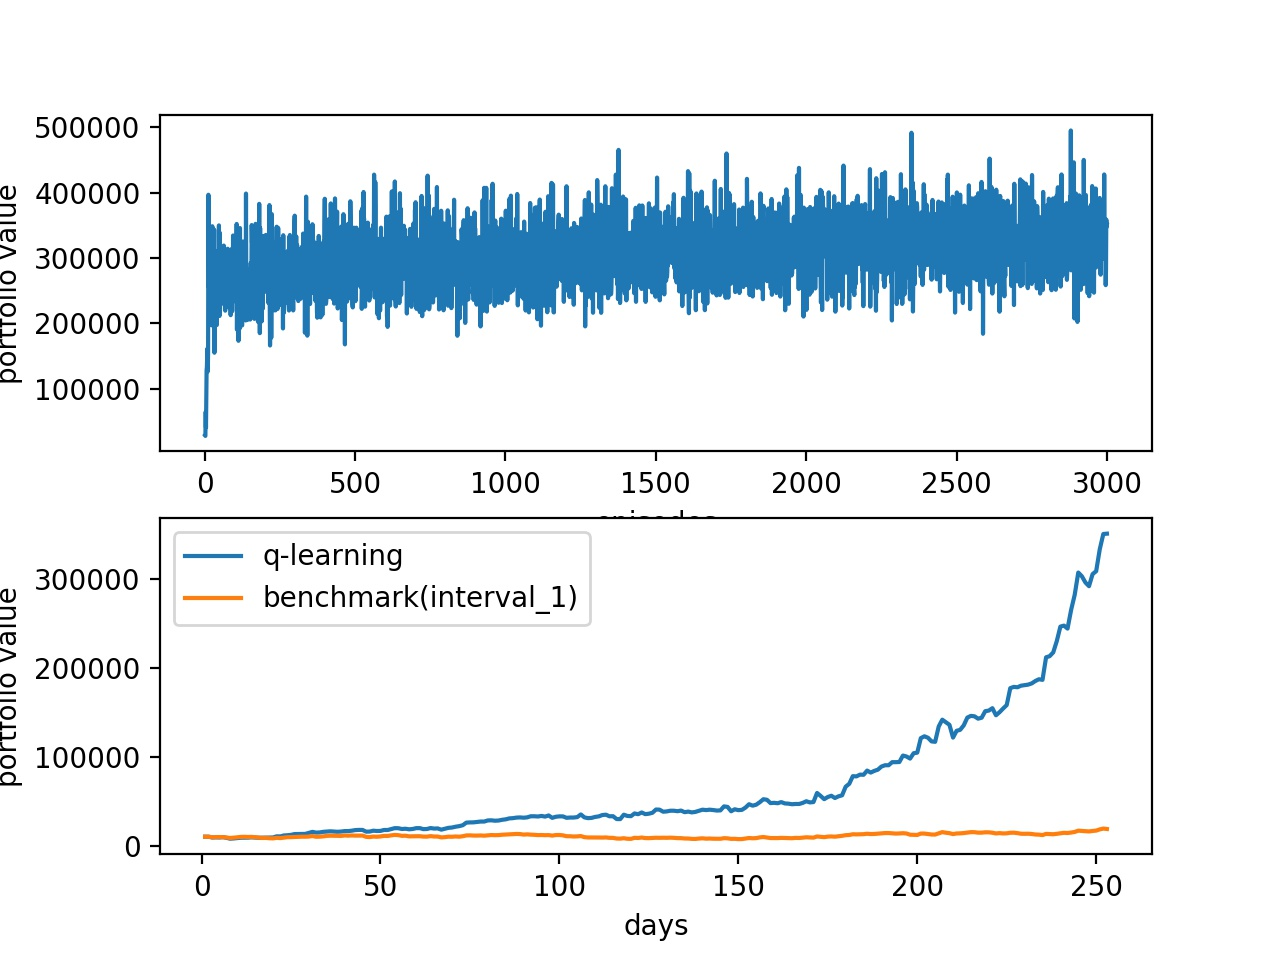
\includegraphics[clip, width=0.6\textwidth]{Graphics/q_learning_KS1.eps} \caption{Training 1 (KLAC \& SKX)}
\end{center}
\end{figure}

\begin{figure}[H]
\begin{center}
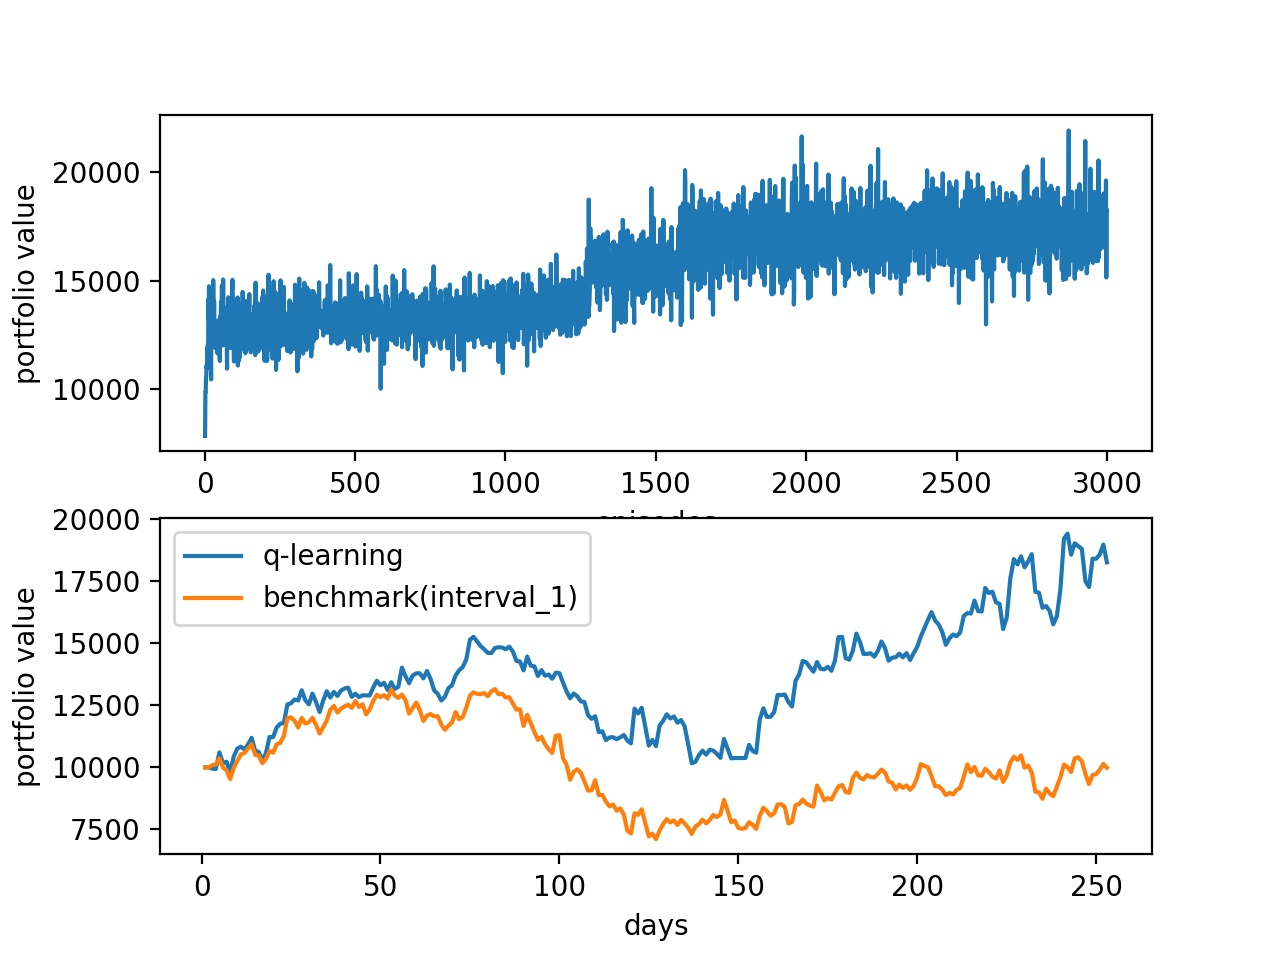
\includegraphics[clip, width=0.6\textwidth]{Graphics/q_learning_MS2.eps} \caption{Training 2 (MU \& SAM)}
\vspace{0.1cm}
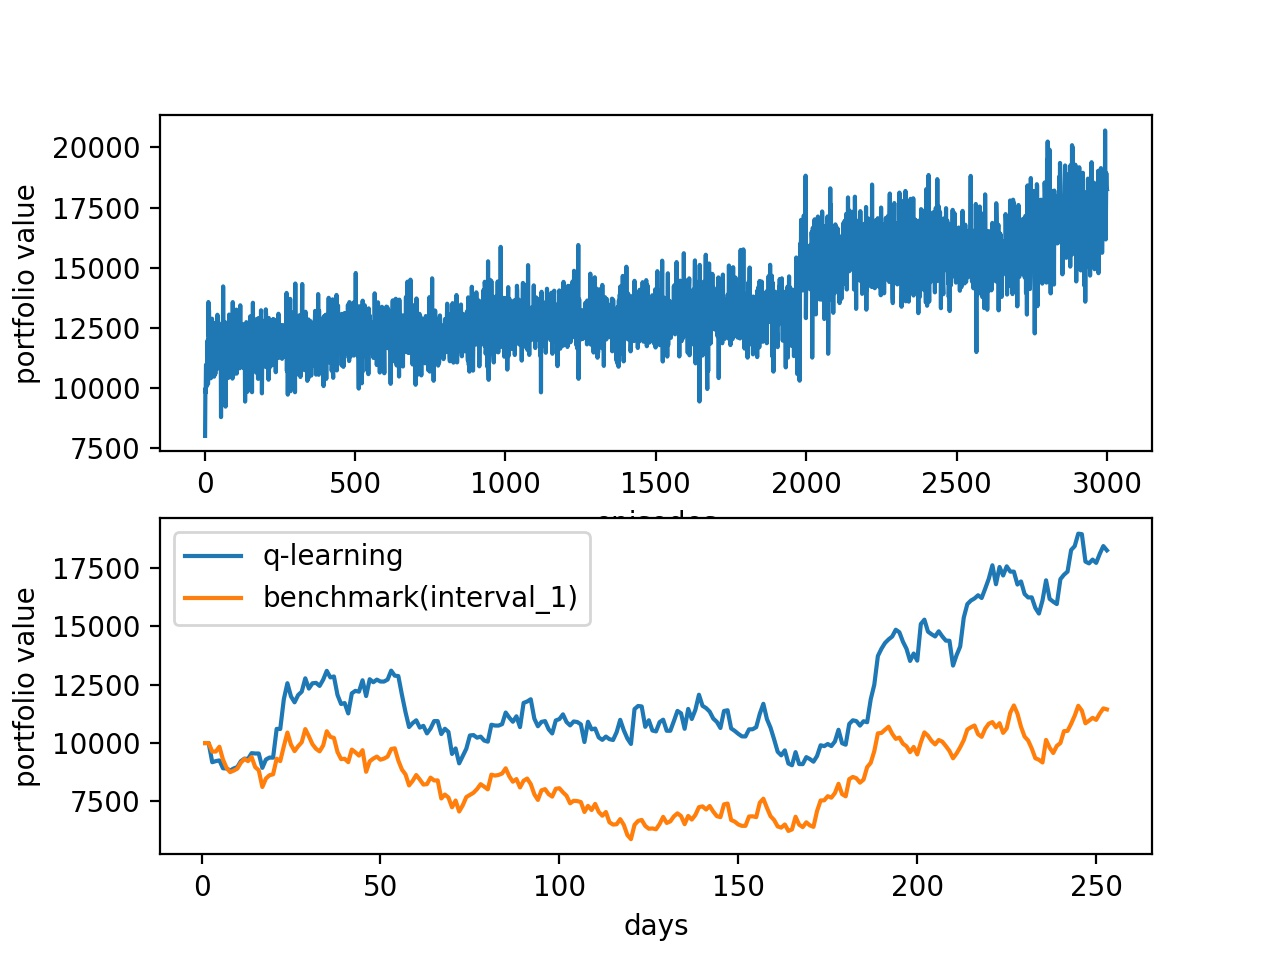
\includegraphics[clip, width=0.6\textwidth]{Graphics/q_learning_LP3.jpg} \caption{Training 3 (LCRX \& PPC)}
\vspace{0.1cm}
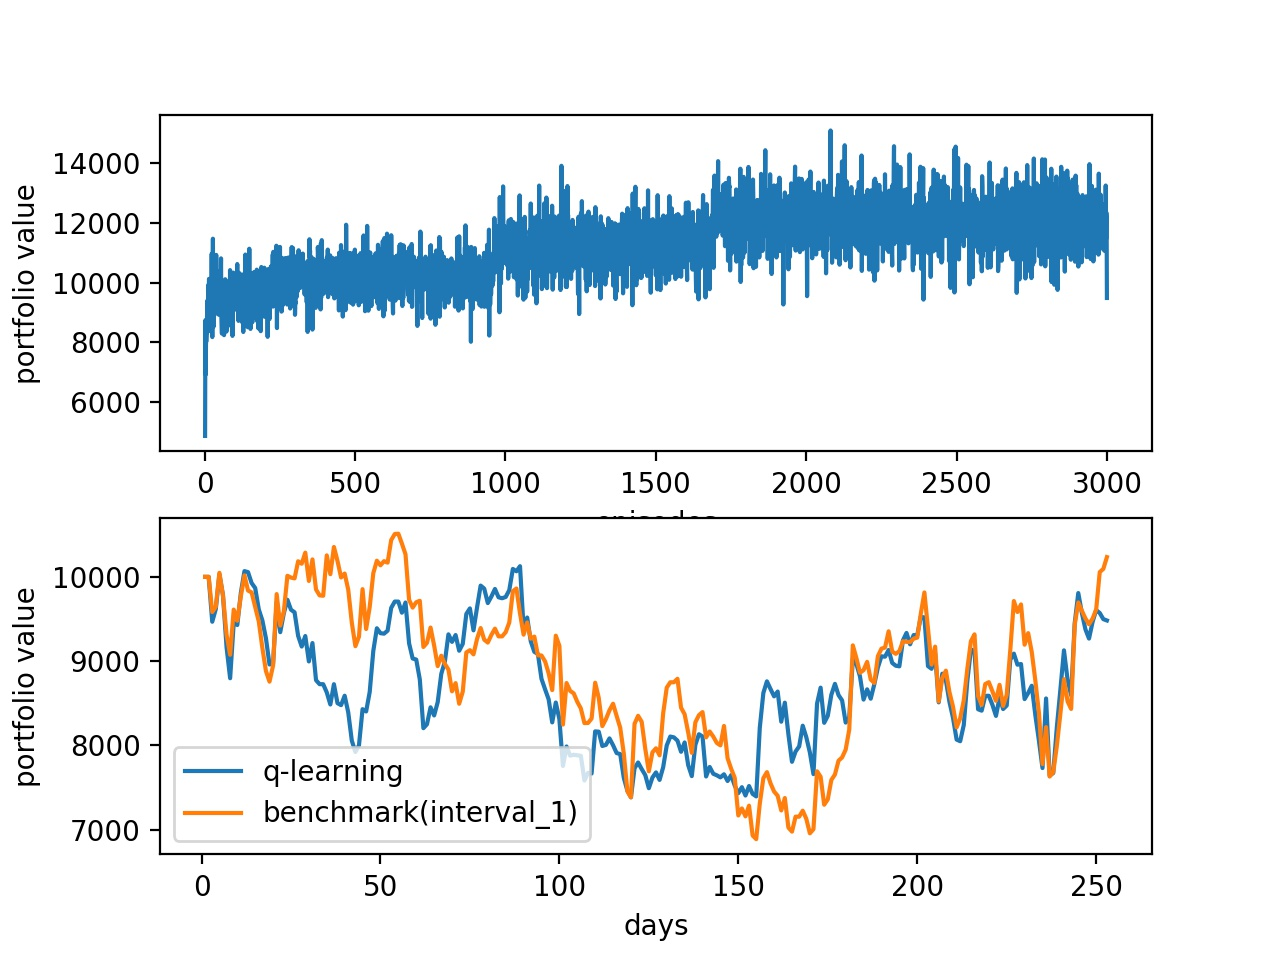
\includegraphics[clip, width=0.6\textwidth]{Graphics/q_learning_AM4.jpg} \caption{Training 4 (AMD \& MTN)}
\end{center}
\end{figure}

\begin{figure}[H]
\begin{center}
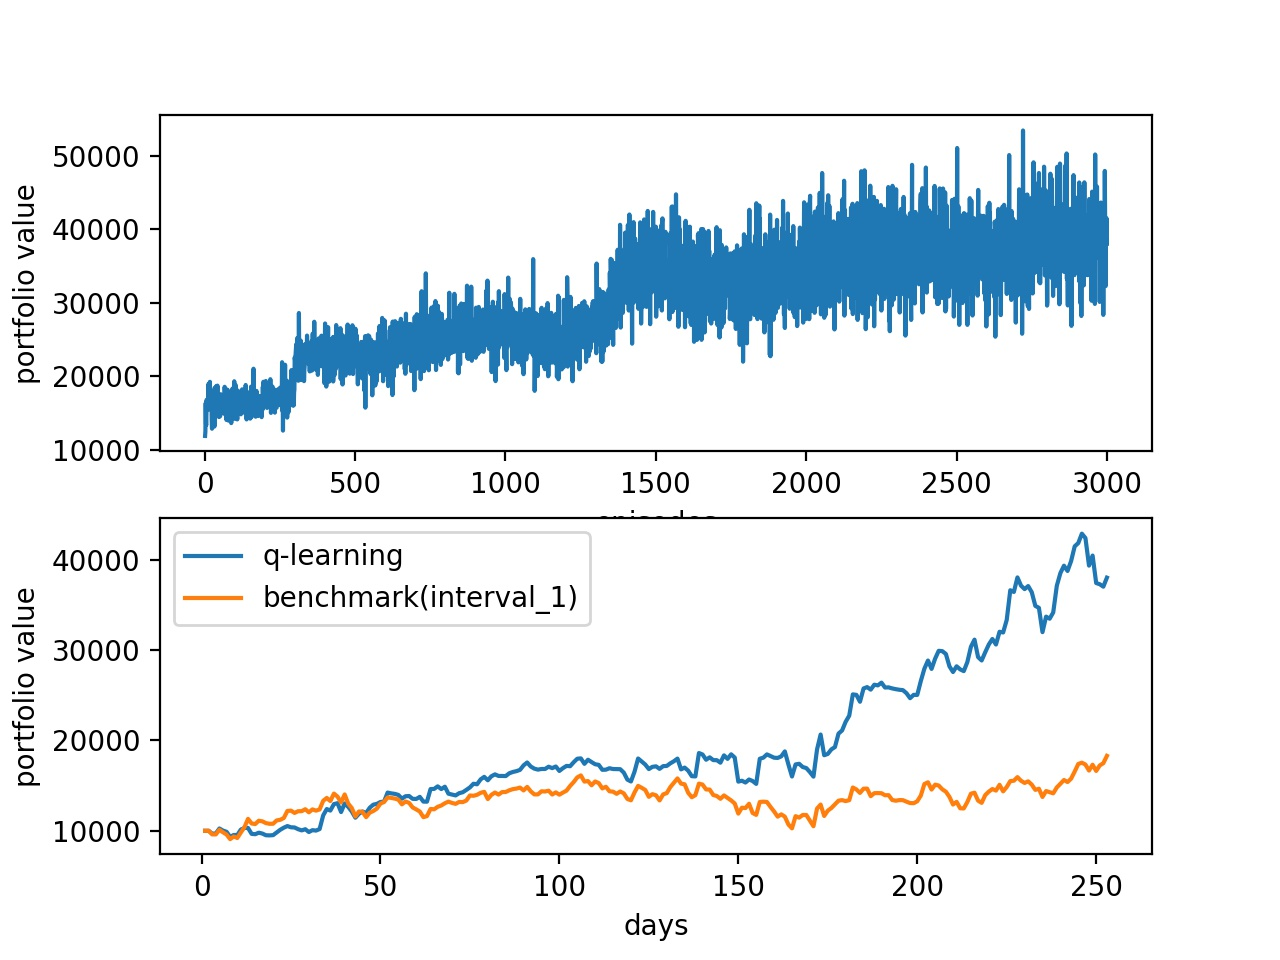
\includegraphics[clip, width=0.6\textwidth]{Graphics/q_learning_NM5.jpg} \caption{Training 5 (NVDA \& MTN)}
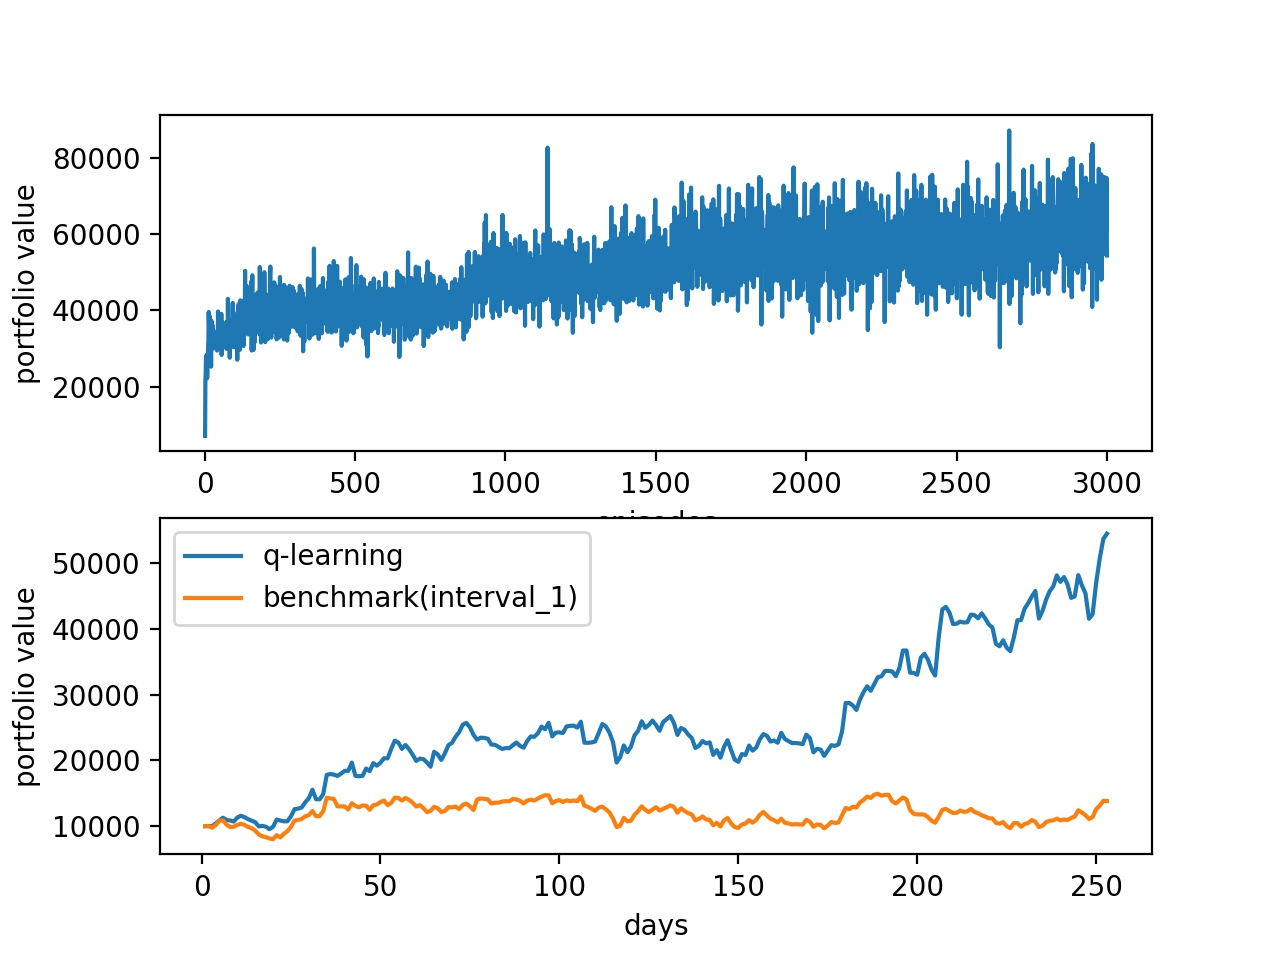
\includegraphics[clip, width=0.6\textwidth]{Graphics/q_learning_IS6.jpg} \caption{Training 6 (INCY \& SKX)}
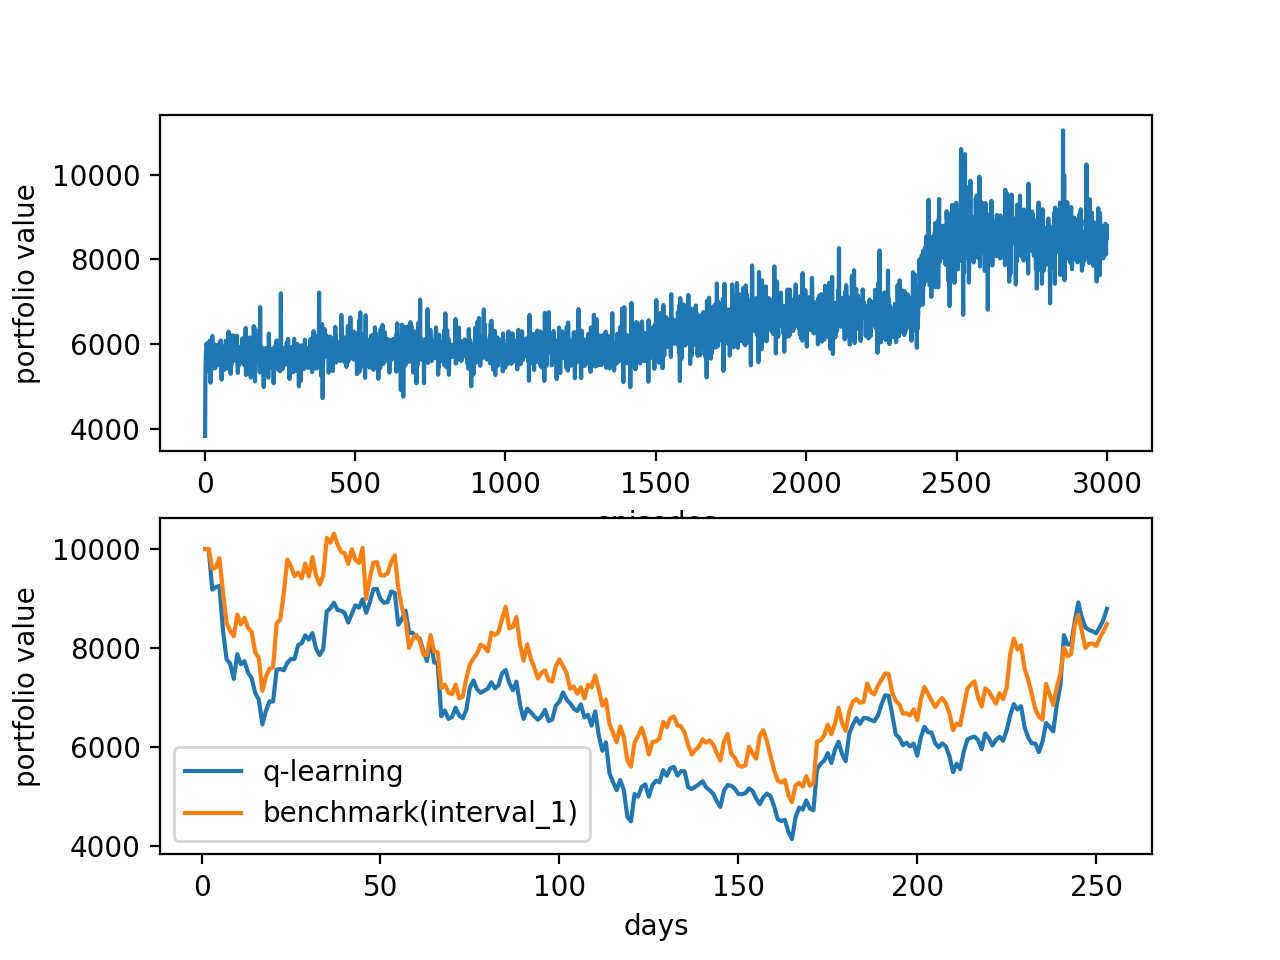
\includegraphics[clip, width=0.6\textwidth]{Graphics/q_learning_LC7.jpg} \caption{Training 7 (LCRX \& CAJ)}
\end{center}
\end{figure}

\begin{figure}[H]
\begin{center}
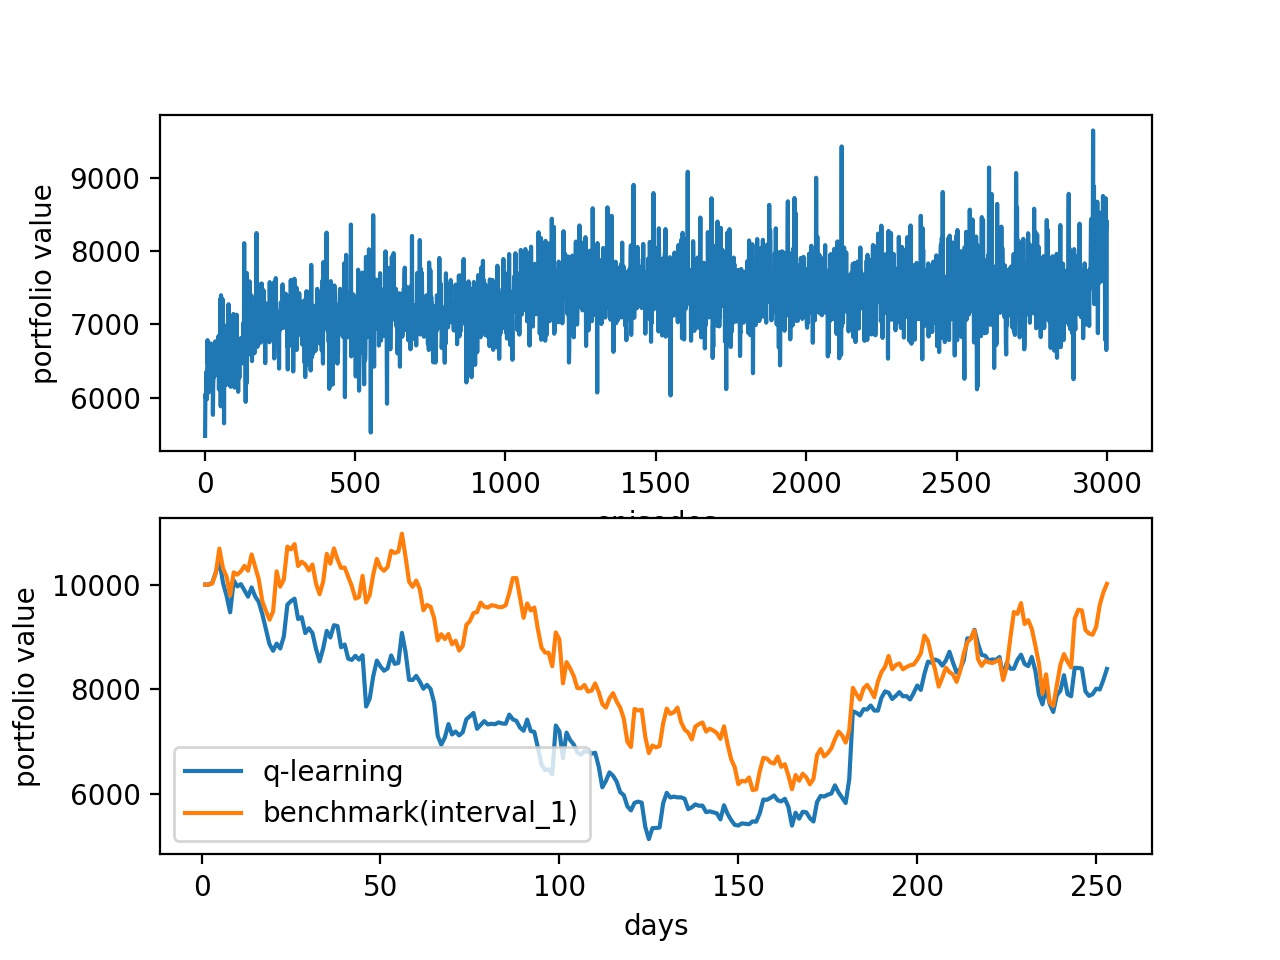
\includegraphics[clip, width=0.6\textwidth]{Graphics/q_learning_AS8.jpg} \caption{Training 8 (AMD \& SAM)}
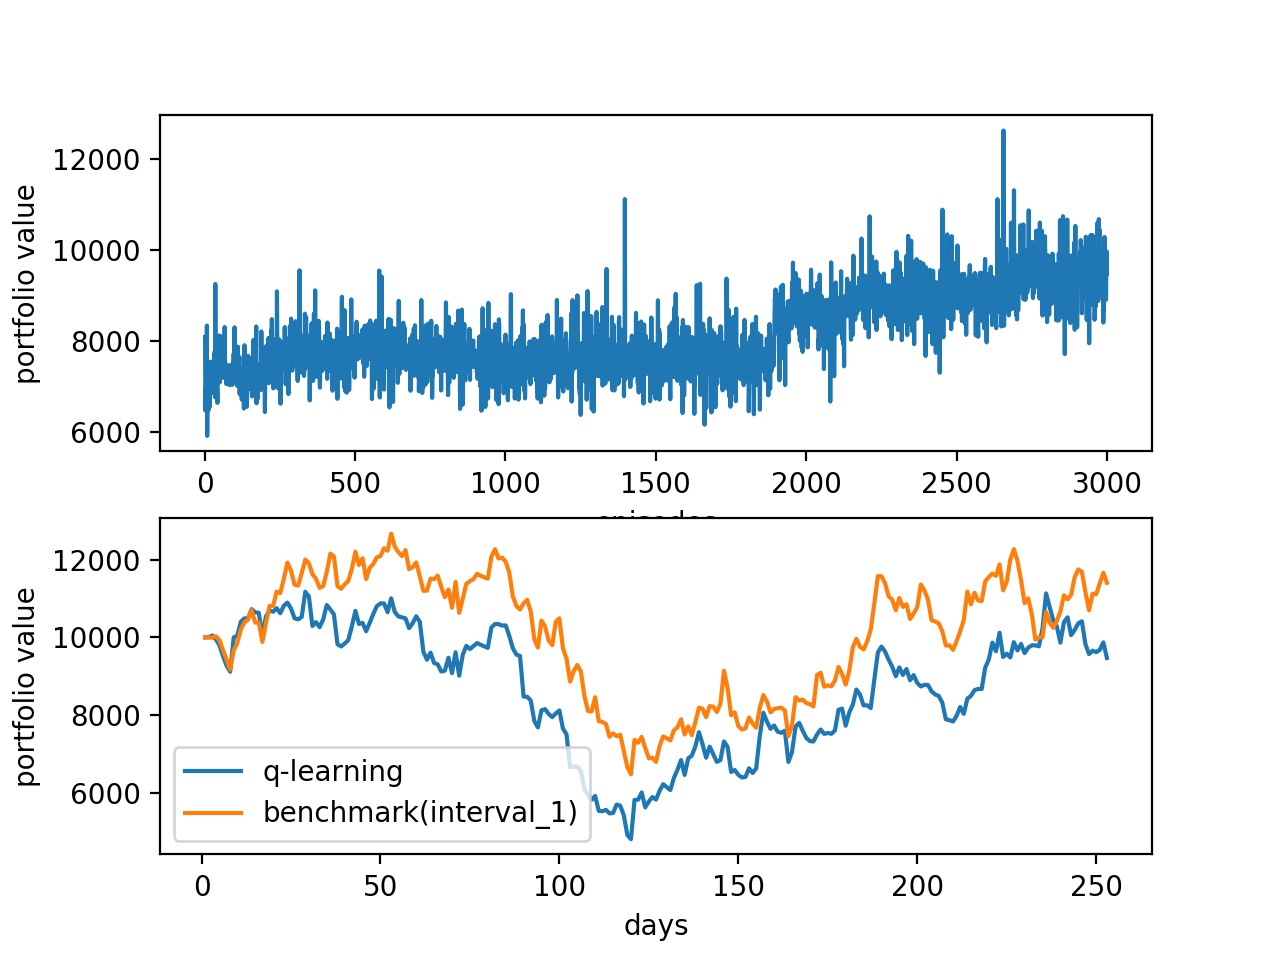
\includegraphics[clip, width=0.6\textwidth]{Graphics/q_learning_MP9.jpg} \caption{Training 9 (MU \& PPC)}
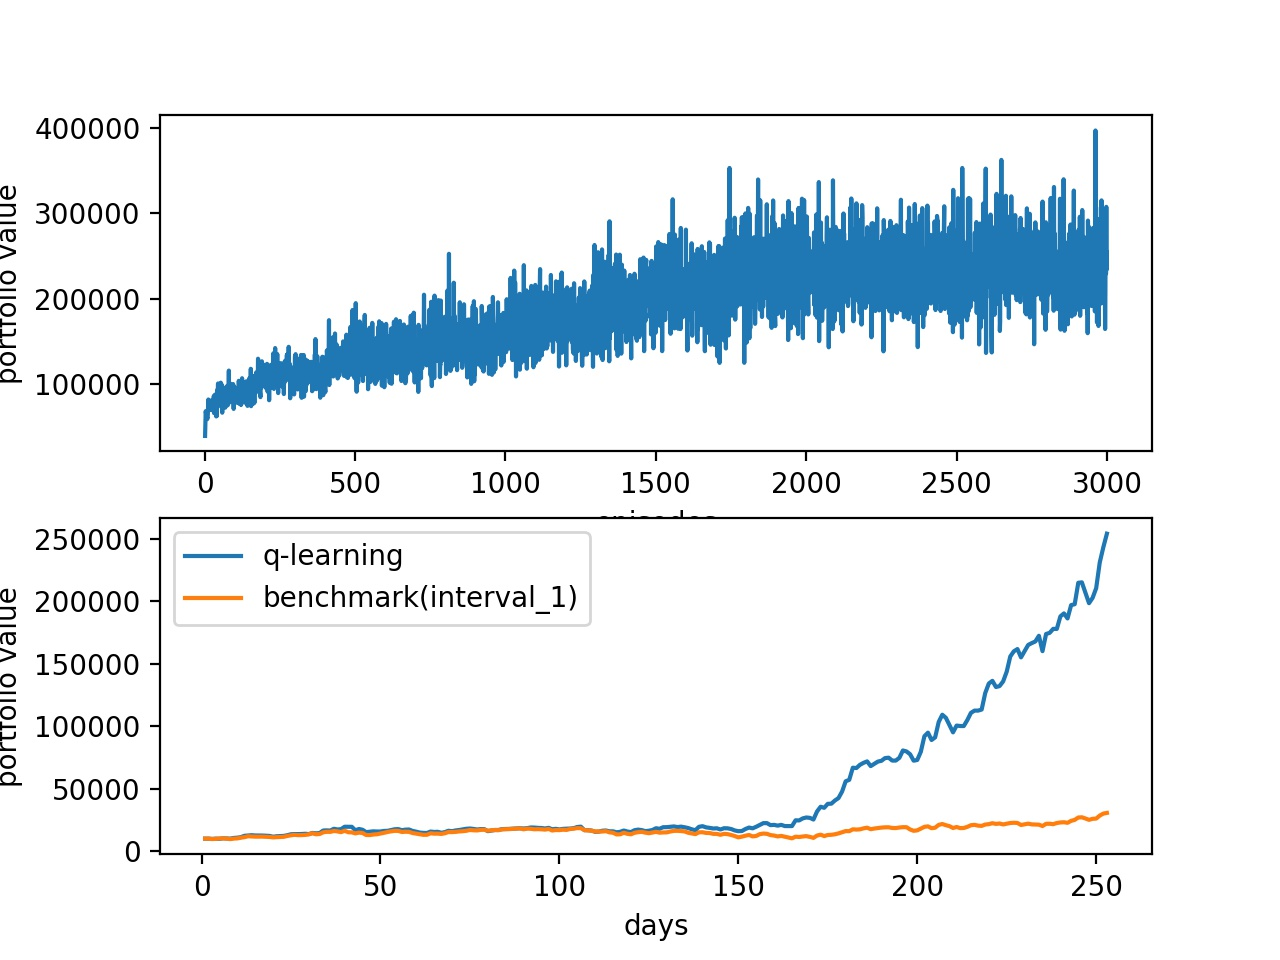
\includegraphics[clip, width=0.6\textwidth]{Graphics/q_learning_NS10.jpg} \caption{Training 10 (NVDA \& SKX)}
\end{center}
\end{figure}

\begin{figure}[H]
\begin{center}
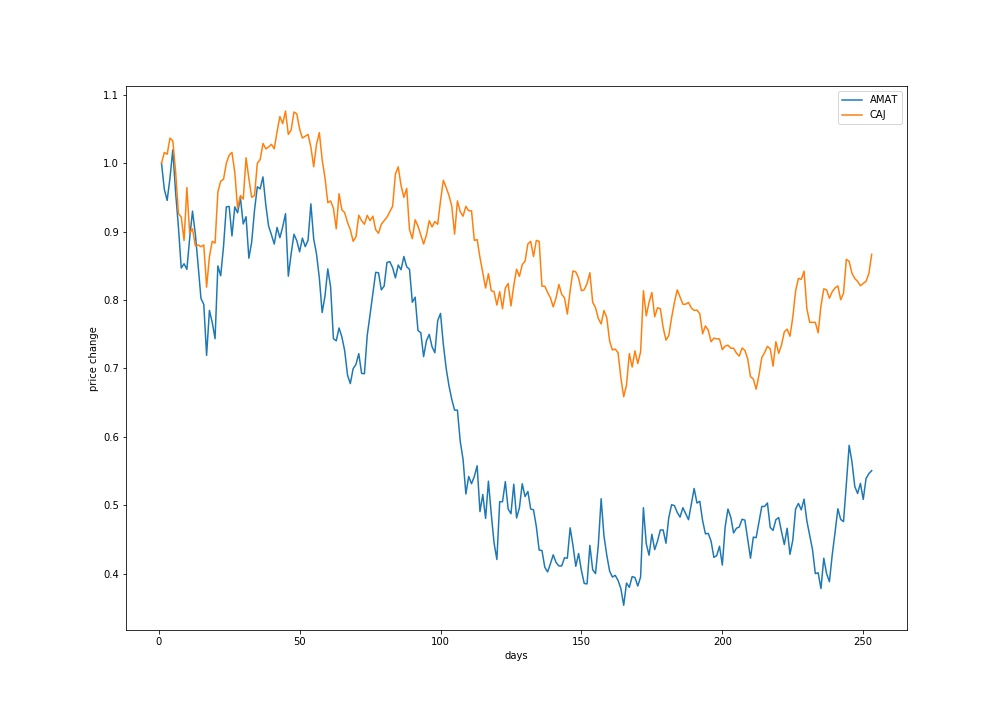
\includegraphics[clip, width=0.6\textwidth]{Graphics/test1_pricechange.jpg} \caption{Test Set1 Price Change AMAT \& CAJ}
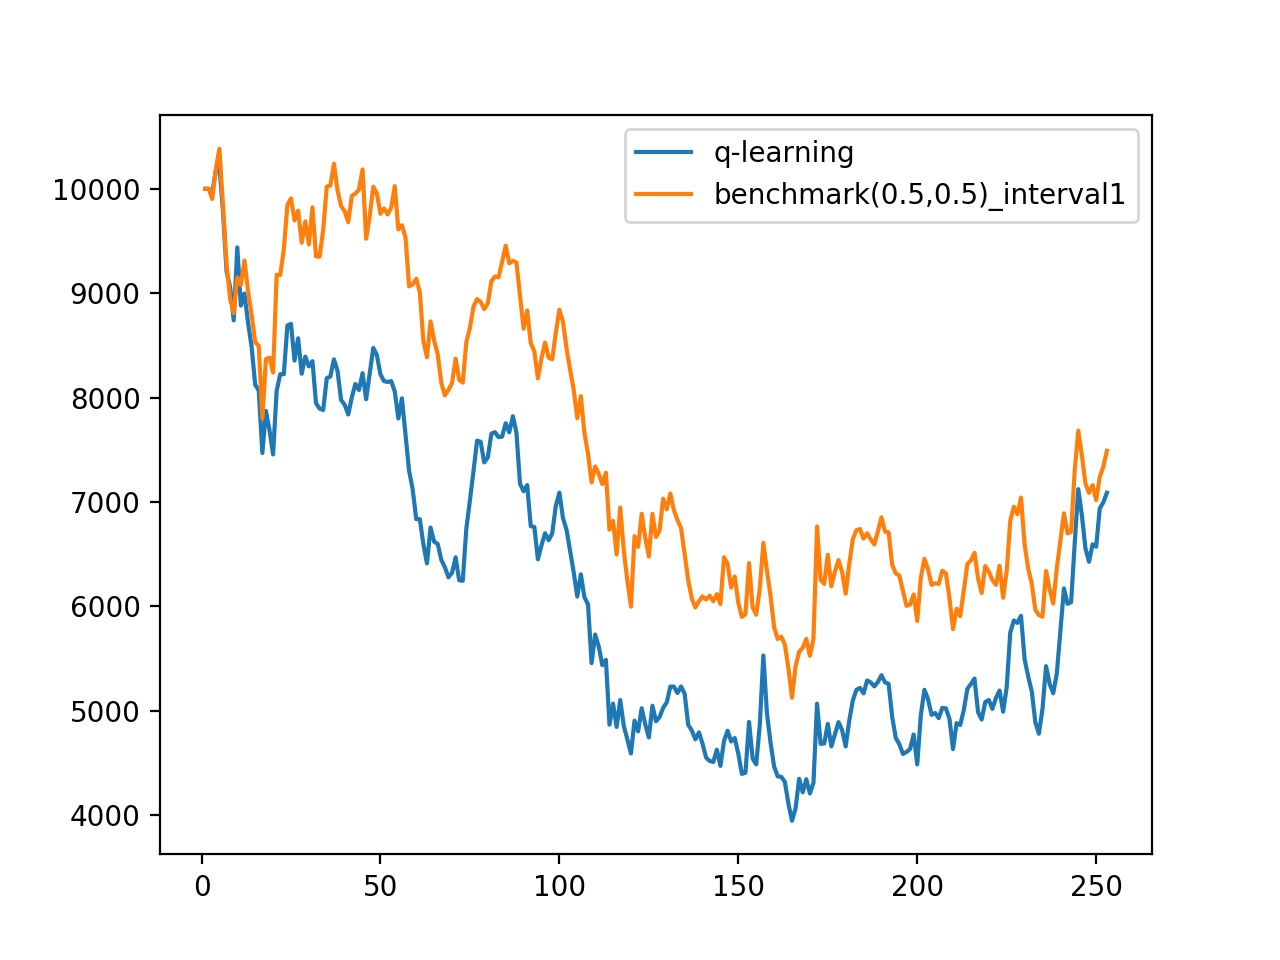
\includegraphics[clip, width=0.6\textwidth]{Graphics/test_KS1_AC_action.jpg} \caption{Test(AMAT \& CAJ) after 1 training}
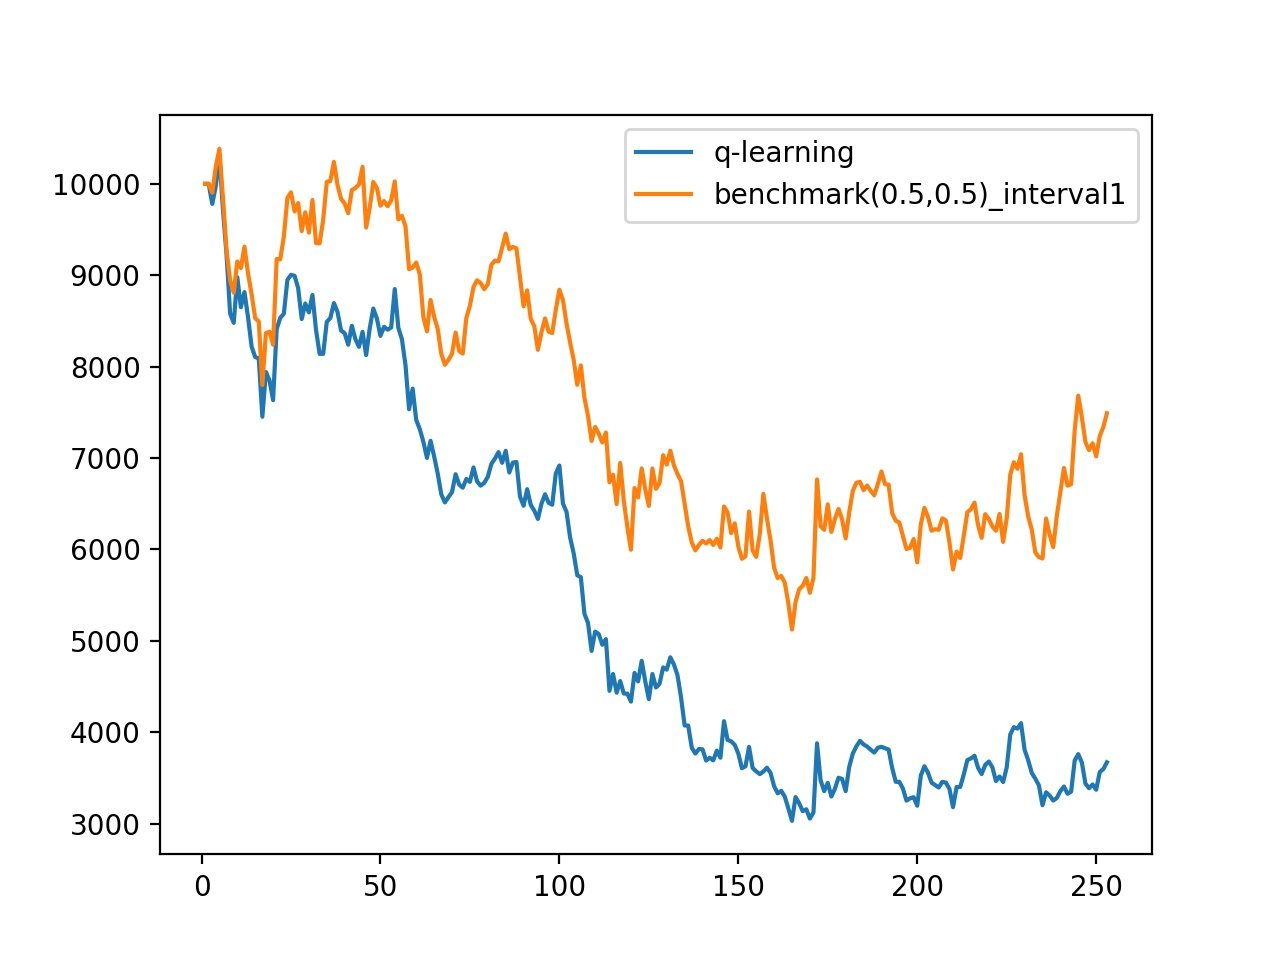
\includegraphics[clip, width=0.6\textwidth]{Graphics/test_LP3_AC_action.jpg} \caption{Test(AMAT \& CAJ) after 3 training
}
\end{center}
\end{figure}

\subsection{Linear Regression}

\section{Deep Q-Network}

\subsection{Including Exchange Ratio}
In the later state of the project, we try to include the exchange ratio into our consideration. The application is that you can include two different countries' stock into the portfolio and settle at the end of the date with one of the stocks' currency in the portfolio. Since sometime due to the difference of public holiday and time-zone in different countries, we may face the situation that one country's stock market is working while the other one is not. When we face such situation, we will just skip that date in our training model.

\endinput
